\documentclass[fleqn,10pt]{wlscirep}
\usepackage[T1]{fontenc}
\usepackage[utf8]{inputenc}
\usepackage{mathptmx}
\usepackage{booktabs,dcolumn}
\usepackage{color, colortbl}
\usepackage{graphicx}
\usepackage{hyperref}
\definecolor{Blue}{rgb}{0.31, 0.51, 0.75}
\definecolor{LightBlue}{rgb}{0.81, 0.85, 0.91}

\bibliographystyle{naturemag-doi}

\title{Machine Learning-Based Identification of Long Non-Coding RNA Signatures for Dual Diagnostic and Prognostic Assessment in Colorectal Cancer}

\author[1]{Zhuha Zhou}
\author[1]{Yongyu Bai}
\author[2]{Qigang Xue}
\author[3]{Zhuxian Zhou}
\author[1*]{Shaolian Han}
\affil[1]{Department of Gastroenterology Surgery, The First Affiliated Hospital of Wenzhou Medical University, Nanbaixiang Street, Ouhai District, 325000, Wenzhou, Zhejiang, China.}
\affil[2]{Department of Hepatobiliary and Pancreatic Surgery, The First Affiliated Hospital of Wenzhou Medical University, Nanbaixiang Street, Ouhai District, 325000, Wenzhou, Zhejiang, China.}
\affil[3]{Center for Bionanoengineering and Key Laboratory of Biomass Chemical Engineering of Ministry of Education, College of Chemical and Biological Engineering, Zhejiang University, Zheda Road 38, 310027, Hangzhou, China.}
\affil[*]{Correspondence and requests for materials should be addressed to S.H. (email: wangguanyu@zju.edu.cn)}

\begin{abstract}
Colorectal cancer (CRC) remains a leading cause of cancer-related mortality, yet clinically actionable molecular biomarkers for early detection and prognosis are still limited. Long non-coding RNAs (lncRNAs) have emerged as promising biomarkers, but identifying robust signatures from high-dimensional transcriptomic data requires systematic computational strategies. Here, we integrate differential expression analysis with elastic-net regularized Cox regression and five machine learning classifiers to discover lncRNA signatures with both diagnostic and prognostic value in CRC. Using the TOIL-recomputed TCGA--GTEx dataset (349 non-tumor, 290 tumor samples) and TCGA-COAD clinical follow-up data (458 patients, 443 with complete survival and expression data), we identified 37 lncRNAs with non-zero coefficients via elastic-net Cox regression and further refined them to a 22-feature model via stepwise multivariate Cox regression. The final risk model incorporating selected lncRNAs and pathological stage stratified patients into distinct risk groups, with time-dependent AUC converging to 0.725 at 8 years. Among classification models, support vector machine (SVM), random forest, and neural network achieved testing-set accuracies of 91.6\%, 92.2\%, and 90.6\%, respectively, substantially outperforming logistic regression (72.8\%) and elastic-net logistic regression (73.3\%). Our findings demonstrate that machine learning-driven analysis of lncRNA expression profiles can yield clinically relevant diagnostic and prognostic biomarkers for CRC, and we provide a fully reproducible, parallelized computational pipeline (v20) as a resource for future biomarker discovery studies.
\end{abstract}

\noindent\textbf{Keywords:} colorectal cancer, long non-coding RNA, machine learning, biomarker, diagnosis, prognosis, Cox proportional hazards, elastic net
\begin{document}
\flushbottom
\maketitle
\thispagestyle{empty}

\section*{Introduction}

Colorectal cancer (CRC) is the third most frequently diagnosed malignancy and the second leading cause of cancer-associated death worldwide, accounting for approximately 1.9 million new cases and 900,000 deaths annually\cite{RN1}. Despite advances in screening and treatment, the majority of CRC cases are diagnosed at advanced stages, when lymph node involvement or distant metastasis has already occurred. The 5-year survival rates decline sharply from 91.1\% for localized disease to 69.8\% for regional spread and 11\% for distant metastasis, highlighting the urgent need for molecular biomarkers that enable early detection and accurate prognosis\cite{RN1}. Alarmingly, CRC incidence among adults under 50 years has been rising since the mid-1990s in many high-income countries, underscoring the importance of developing novel diagnostic and prognostic tools.

Long non-coding RNAs (lncRNAs) are transcripts longer than 200 nucleotides that do not encode proteins but function as versatile regulators of gene expression at the epigenetic, transcriptional, and post-transcriptional levels. Accumulating evidence has demonstrated that lncRNAs participate in cancer hallmarks including proliferation, invasion, metastasis, and drug resistance\cite{RN3}, and several lncRNAs have been specifically implicated in CRC pathogenesis through diverse mechanisms\cite{RN4,RN5,RN6}. Because lncRNAs exhibit tissue-specific and disease-specific expression patterns, they are increasingly recognized as promising biomarkers and therapeutic targets\cite{RN7,RN8,RN9}. However, traditional experimental approaches for discovering disease-associated lncRNAs are time-consuming and low-throughput, creating a strong incentive for computational methods that can prioritize candidates from large-scale sequencing data.

The public availability of RNA-sequencing datasets from The Cancer Genome Atlas (TCGA)\cite{RN10} and the Genotype-Tissue Expression (GTEx)\cite{RN11} projects has created unprecedented opportunities for transcriptome-wide biomarker discovery. Notably, the TOIL project developed by the University of California, Santa Cruz, has recomputed TCGA and GTEx raw expression data through a unified pipeline, minimizing batch effects and enabling direct comparison between tumor and normal tissues\cite{RN12}. This harmonized resource provides a statistically well-powered foundation for identifying differentially expressed lncRNAs that distinguish CRC from normal tissue, particularly because the original TCGA-COAD cohort contains only 41 adjacent non-tumor samples, which is insufficient for robust differential expression analysis.

Machine learning has emerged as a transformative tool in CRC research, with applications spanning colonoscopy screening, histopathological diagnosis, radiomics-based prognostication, and genomic biomarker discovery\cite{RN13}. Supervised classification algorithms can distinguish cancerous from normal tissues with high accuracy, while survival models estimate patient risk over time\cite{RN14,RN15}. Despite these advances, the application of machine learning to lncRNA-based biomarker discovery remains relatively underexplored. The \texttt{caret} package in R provides a unified interface that streamlines model training, hyperparameter tuning, and performance evaluation across diverse algorithms\cite{RN16}. Zhang \textit{et al.} developed CRlncRC, a machine learning-based classifier for cancer-related lncRNAs that integrates multiple optimization strategies\cite{RN17}. However, studies that simultaneously assess diagnostic and prognostic utility of lncRNA signatures using standardized, reproducible machine learning pipelines remain scarce\cite{RN18}. Although machine learning holds tremendous promise for medical applications, translating computational models into clinically actionable tools requires rigorous validation and attention to interpretability\cite{RN19}.

In this study, we designed an integrated computational pipeline to identify lncRNA signatures with dual diagnostic and prognostic value in CRC. Our pipeline combines differential expression analysis across the harmonized TCGA--GTEx dataset, elastic-net regularized Cox regression for feature selection, multivariate Cox proportional hazards modeling and random survival forests for prognostic evaluation, and five classification algorithms for diagnostic prediction. The identified lncRNA panel yielded excellent discriminative performance in distinguishing tumor from normal tissue and provided stable, time-dependent prognostic stratification beyond routine pathological staging.

\section*{Results}

\subsection*{Identification of candidate lncRNAs through differential expression and survival analysis}

We developed a computational pipeline to systematically identify lncRNAs with diagnostic and prognostic potential in CRC (Fig.~\ref{Fig1}). Starting from 58,387 genes in the TOIL-recomputed TCGA--GTEx colon dataset (349 non-tumor and 290 tumor samples), we removed lowly expressed genes (value $< 0.1$ in $> 60\%$ of samples), retaining 27,560 genes. From these, we extracted lncRNA annotations using GENCODE v22 and v23 references, yielding 15,900 (v22) and 15,931 (v23) lncRNA transcripts respectively.

For prognostic analysis, we used the TCGA-COAD HTSeq-FPKM expression dataset (456 primary tumor samples) together with clinical follow-up data from 458 patients, of whom 443 had complete survival, stage, and lncRNA expression information. After intersecting with lncRNA annotations, 799 lncRNAs were available for survival analysis. We performed univariate Cox proportional hazards regression and Kaplan--Meier log-rank tests for each lncRNA against overall survival (OS). This identified 72 lncRNAs with significant univariate Cox associations ($p < 0.05$).

For feature selection, we applied elastic-net regularized Cox regression with tenfold cross-validation across an $\alpha$ grid (0 to 1 by 0.1). To improve computational efficiency while retaining biological signal, we retained the top 100 lncRNAs ranked by expression variance across patients. The elastic-net procedure identified 37 lncRNAs with non-zero coefficients (Fig.~\ref{Fig2}). These candidates were further refined via stepwise multivariate Cox regression (bidirectional selection minimizing AIC) on the training set, yielding a final model of 22 features that achieved an AIC of 593.46 and C-index of 0.82 (Fig.~\ref{Fig3}).

The differential expression and survival analysis results for the 17 most prominent candidate lncRNAs (ranked by Cox hazard ratio) are summarized in Table~\ref{Tab1}. The majority were significantly downregulated in tumor tissue and associated with increased hazard ratios. Two lncRNAs showed the opposite pattern: AC114730.3 ($\log_2$FC = 1.688, HR = 0.87) and LINC00261 ($\log_2$FC = 3.045, HR = 0.90) were upregulated in tumor tissue yet associated with decreased hazard ratios, consistent with reported tumor-suppressive roles.

\begin{figure}[!htp]
\centering
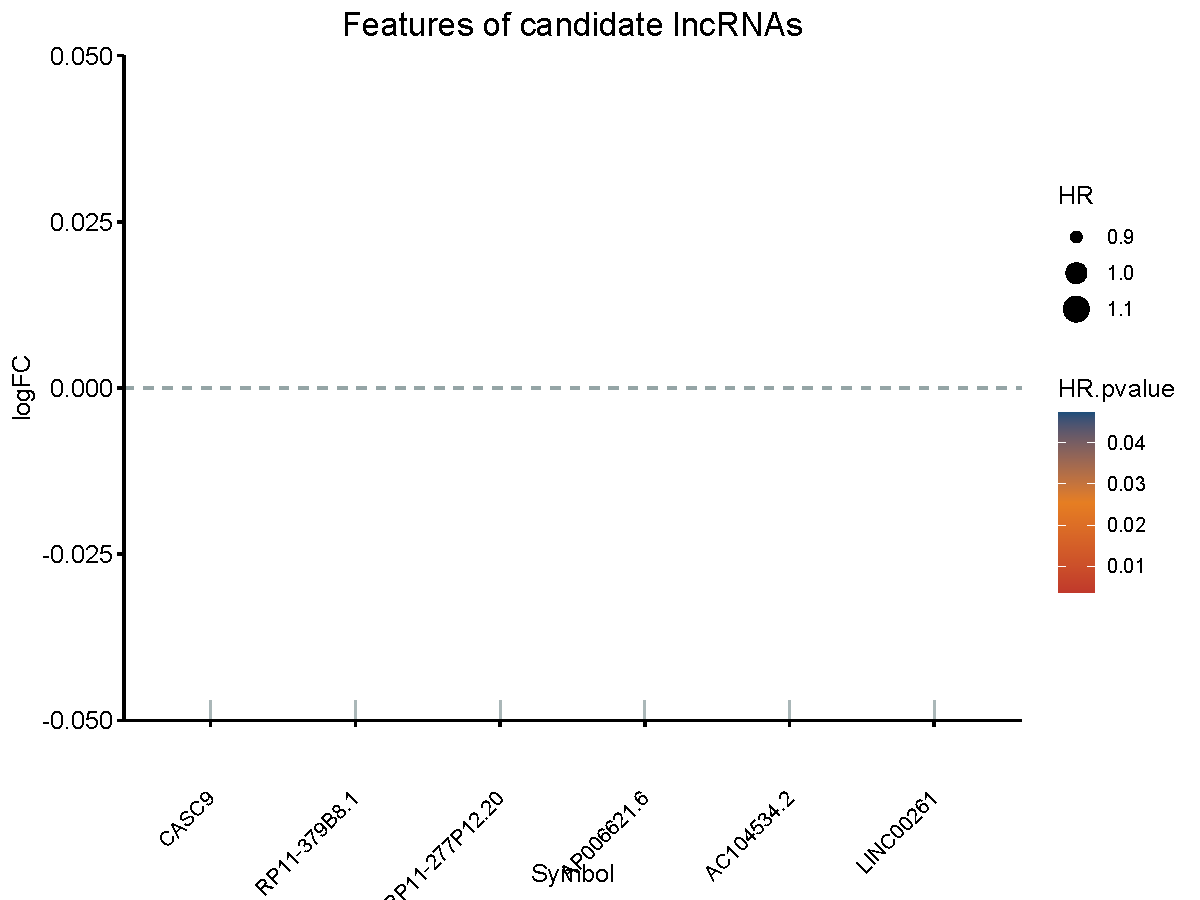
\includegraphics[width=0.92\textwidth, keepaspectratio]{Fig1_candidates}
\caption{Features of candidate lncRNAs. Dot chart showing the 37 lncRNAs selected by elastic-net regularized Cox regression, ranked by log$_2$ fold-change with dot size proportional to hazard ratio and color indicating Cox $p$-value. The TOIL-recomputed TCGA--GTEx expression data ($\log_2(\text{FPKM}+0.001)$ normalized, $n = 639$ samples) were used for differential expression analysis and classification model construction. The TCGA-COAD follow-up survival data ($n = 458$ patients) informed prognostic model development.}
\label{Fig1}
\end{figure}

\begin{table}[!htp]
  \setlength\tabcolsep{3pt}
  \centering
  \extrarowheight=\aboverulesep
    \addtolength{\extrarowheight}{\belowrulesep}
    \aboverulesep=0pt
    \belowrulesep=0pt
  \caption{Differential expression and univariate survival analysis of the 17 candidate lncRNAs.}
    \begin{tabular}{lccccccc}
    \toprule[2pt]
   \rowcolor{Blue} \textbf{Symbol} & \textbf{Ensembl ID} &\textbf{$\log_{2}$FC}
     &\textbf{ FDR} &\textbf{ HR }   &\textbf{ 95\% CI}    & \textbf{$p$-value} & \textbf{Log-rank $p$}\\
    \midrule[1pt]
   ARRDC1-AS1 & ENSG00000203993.4 & -0.745 & $<0.001$ & 1.80 & (1.21--2.65) & 0.003 & 0.008 \\
    \specialrule{0em}{.02em}{.02em}
   \rowcolor{LightBlue}  EIF3J-AS1 & ENSG00000179523.4 & -0.387 & $<0.001$ & 1.70 & (1.20--2.53) & 0.004 & 0.037 \\
     \specialrule{0em}{.02em}{.02em}
  CTB-25B13.12 & ENSG00000267317.2 & 0.014 & 0.888 & 1.70 & (1.28--2.36) & $<0.001$ & 0.002 \\
     \specialrule{0em}{.02em}{.02em}
    \rowcolor{LightBlue}  AP006621.5 & ENSG00000255284.1 & -1.114 & $<0.001$ & 1.60 & (1.22--2.01) & $<0.001$ & 0.134 \\
 \specialrule{0em}{.02em}{.02em}
  RP11-644F5.11 & ENSG00000258056.2 & -0.327 & 0.001 & 1.60 & (1.15--2.34) & 0.007 & 0.037 \\
    \specialrule{0em}{.03em}{.03em}
     \rowcolor{LightBlue} AC113189.5 & ENSG00000233223.2 & -0.734 & $<0.001$ & 1.50 & (1.20--1.92) & 0.001 & 0.218 \\
 \specialrule{0em}{.02em}{.02em}
RP11-44M6.7 & ENSG00000274272.1 & -1.254 & $<0.001$  & 1.50 & (1.18--2.02) & 0.002 & 0.010 \\
 \specialrule{0em}{.02em}{.02em}
     \rowcolor{LightBlue} LINC00174 & ENSG00000179406.6 & -1.016 & $<0.001$  & 1.40 & (1.11--1.72) & 0.004 & 0.052 \\
   \specialrule{0em}{.02em}{.02em}
  TNRC6C-AS1 & ENSG00000204282.4 & -0.140 & 0.213 & 1.40 & (1.10--1.78) & 0.006 & 0.018 \\
 \specialrule{0em}{.02em}{.02em}
   \rowcolor{LightBlue}   MIR210HG & ENSG00000247095.2 & 0.129 & 0.352 & 1.40 & (1.17--1.68) & $<0.001$ & 0.006 \\
    \specialrule{0em}{.03em}{.03em}
     RP11-199F11.2 & ENSG00000262251.1 & 0.244 & 0.022 & 1.40 & (1.10--1.78) & 0.006 & 0.025 \\
 \specialrule{0em}{.02em}{.02em}
     \rowcolor{LightBlue} RP5-1021I20.1 & ENSG00000259065.1 & -1.029 & $<0.001$  & 1.30 & (1.07--1.52) & 0.007 & 0.007 \\
     \specialrule{0em}{.03em}{.03em}
  RP11-268J15.5 & ENSG00000116883.8 & -0.409 & 0.001 & 1.20 & (1.06--1.38) & 0.005 & 0.002 \\
 \specialrule{0em}{.02em}{.02em}
    \rowcolor{LightBlue}  AC156455.1 & ENSG00000256546.1 & -0.948 & $<0.001$ & 1.20 & (1.05--1.35) & 0.007 & 0.089 \\
 \specialrule{0em}{.02em}{.02em}
   RP11-440D17.3 & ENSG00000272913.1 & -0.232 & 0.152 & 1.10 & (0.91--1.19) & 0.064 & 0.200 \\
  \specialrule{0em}{.02em}{.02em}
    \rowcolor{LightBlue}  LINC00261 & ENSG00000259974.2 & 3.045 & $<0.001$  & 0.90 & (0.82--0.98) & 0.022 & 0.035 \\
 \specialrule{0em}{.02em}{.02em}
   AC114730.3 & ENSG00000224272.2 & 1.688 & $<0.001$   & 0.87 & (0.79--0.97) & 0.012 & 0.074 \\
    \bottomrule[1.5pt]
    \end{tabular}
  \label{Tab1}
\end{table}

\begin{figure}[htp]
\centering
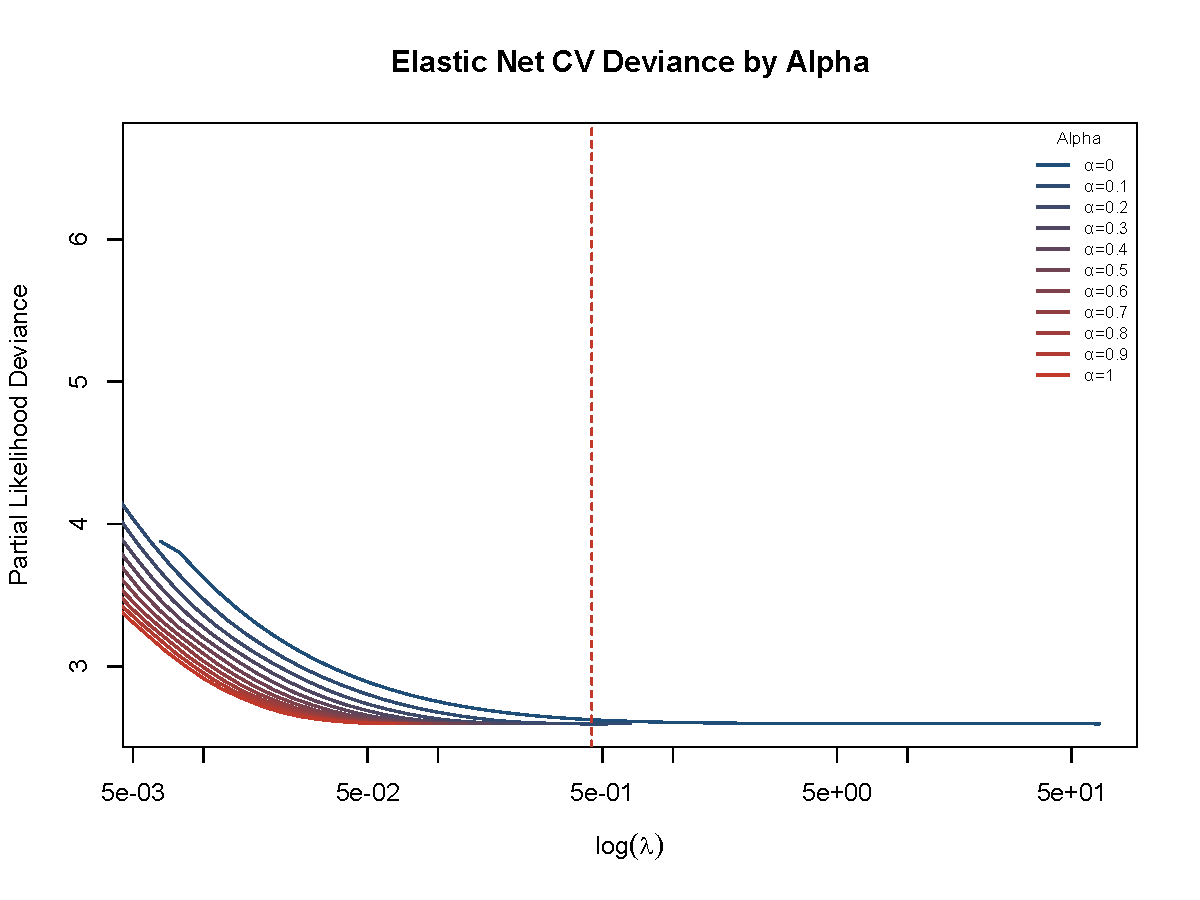
\includegraphics[width=1\columnwidth, keepaspectratio]{Fig2a_deviance}
\caption{Elastic-net regularized Cox regression hyperparameter tuning. \textbf{(a)} Tenfold cross-validated partial log-likelihood deviance surface as a function of mixing parameter $\alpha$ and $\log(\lambda)$. \textbf{(b)} Coefficient shrinkage paths; red paths correspond to the 37 lncRNAs with non-zero coefficients at the optimal $\lambda$.}
\label{Fig2}
\end{figure}

\subsection*{Prognostic model construction and survival prediction}

We randomly partitioned the follow-up survival data into training (70\%, n=300) and testing (30\%, n=128) sets, preserving balanced distributions of survival status and clinical features (Table~S1). Because a substantial proportion of clinical covariates contained missing values, only pathological stage—a well-established prognostic factor—was included alongside lncRNA expression in downstream models. Stage was treated as an ordinal categorical covariate with dummy coding and stage I as the reference level.

We further refined the 37 elastic-net-selected lncRNAs via stepwise multivariate Cox regression (bidirectional selection) on the training set. The final model, comprising 22 features (including pathological stage), achieved an Akaike information criterion (AIC) of 593.46, a concordance index (C-index) of 0.82, and a highly significant global likelihood-ratio test ($p < 10^{-11}$). The key predictors—including MIR210HG, EIF3J-AS1, RP11-440D17.3, and stage IV—showed significantly elevated hazard ratios consistent with earlier findings (Fig.~\ref{Fig3}).

\begin{figure}[htp]
\centering

\includegraphics[width=1\textwidth]{Fig3_forest}
\caption{Forest plot of the stepwise multivariate Cox proportional hazards model. Hazard ratios with 95\% confidence intervals and Wald test $p$-values are shown for the 22 features (including pathological stage) retained in the final model. Stage I served as the reference category. The key predictors with significantly elevated hazard ratios are highlighted.}
\label{Fig3}
\end{figure}

We computed the relative risk score (RRS) for each patient as the prognostic index $\beta^T\mathbf{X}$ relative to the population average, and stratified patients into high- and low-risk groups using the median RRS as the threshold. The RRS was significantly higher among patients who died of CRC in both the training and testing sets (Fig.~S1b). In the combined cohort, 73 out of 94 deceased patients (77.7\%) were classified as high-risk, compared to 21 (22.3\%) classified as low-risk (Table~S2). Kaplan--Meier analysis demonstrated clear separation between risk groups (Fig.~\ref{Fig4}a, b), with log-rank $p < 0.0001$ in the training set and $p = 0.0028$ in the testing set. Patient-level risk score distributions confirmed that deceased and high-risk patients were predominantly concentrated in the upper-risk region (Fig.~S1c).

The RRS also served as an effective metric for time-dependent risk prediction. Time-dependent receiver operating characteristic (ROC) analysis showed that the area under the curve (AUC) converged to approximately 0.725 in both training and testing sets after 8 years of follow-up (Fig.~\ref{Fig5}). The moderate fluctuation observed during the initial years likely reflects the low event rate in early follow-up.

For comparison, we also constructed a random survival forest (RSF) model using the same eight lncRNAs and stage. The RSF was tuned to optimal hyperparameters ($\text{ntree} = 500$, $\text{nodesize} = 60$, $\text{mtry} = 1$) on the training data, with tree splitting based on the log-rank statistic. The RSF achieved an out-of-bag (OOB) error of 25.011\% on the training set but generalized less effectively, with an OOB error of 32.169\% on the testing set (Fig.~\ref{Fig4}c, d). The time-dependent Brier score, which quantifies prediction error, increased gradually over follow-up time in both models. The Cox model consistently produced lower prediction errors than the RSF across all time points (Fig.~\ref{Fig6}a, b). The C-index remained stable over time for both models, with the Cox model achieving superior discrimination. Notably, incorporating the eight lncRNAs improved prediction performance relative to a Cox model with stage alone, confirming the additive prognostic value of the lncRNA signature (Fig.~\ref{Fig6}c, d).

\begin{figure}[htp]
\centering

\includegraphics[width=1\textwidth]{Fig4a_km_train}
\caption{Survival risk stratification by Cox proportional hazards model. Kaplan--Meier curves for high- and low-risk groups stratified by median relative risk score in the training (left) and testing (right) sets. Log-rank $p$-values indicate significant separation between risk groups in both cohorts.}
\label{Fig4}
\end{figure}

\begin{figure}[htp]
\centering
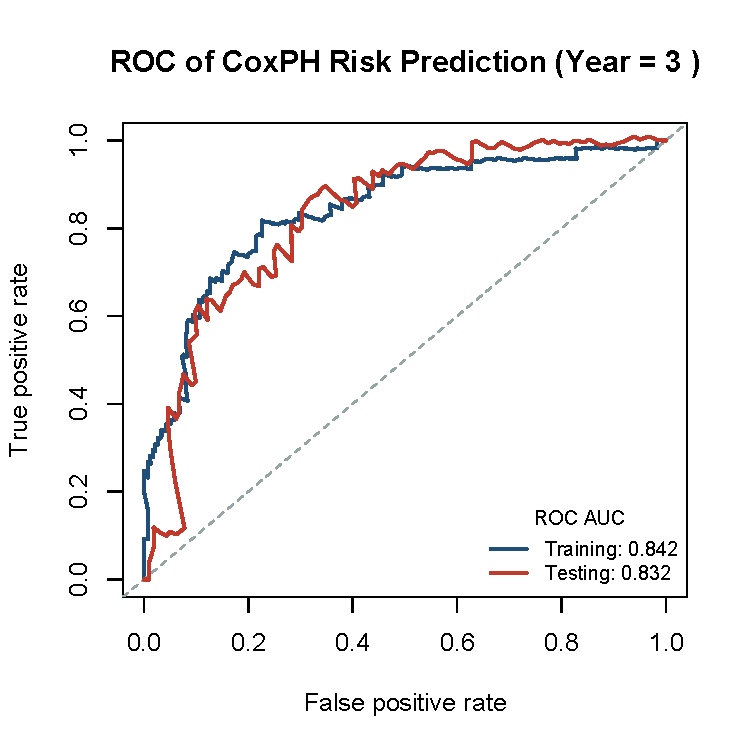
\includegraphics[width=1\textwidth]{Fig5a_roc}
\caption{Time-dependent ROC analysis of the relative risk score. ROC curves showing sensitivity and specificity of the RRS for predicting survival at 3-year and 5-year time points in training and testing sets. The time-dependent AUC trajectory converges to approximately 0.725 after 8 years of follow-up.}
\label{Fig5}
\end{figure}

\begin{figure}[htp]
\centering
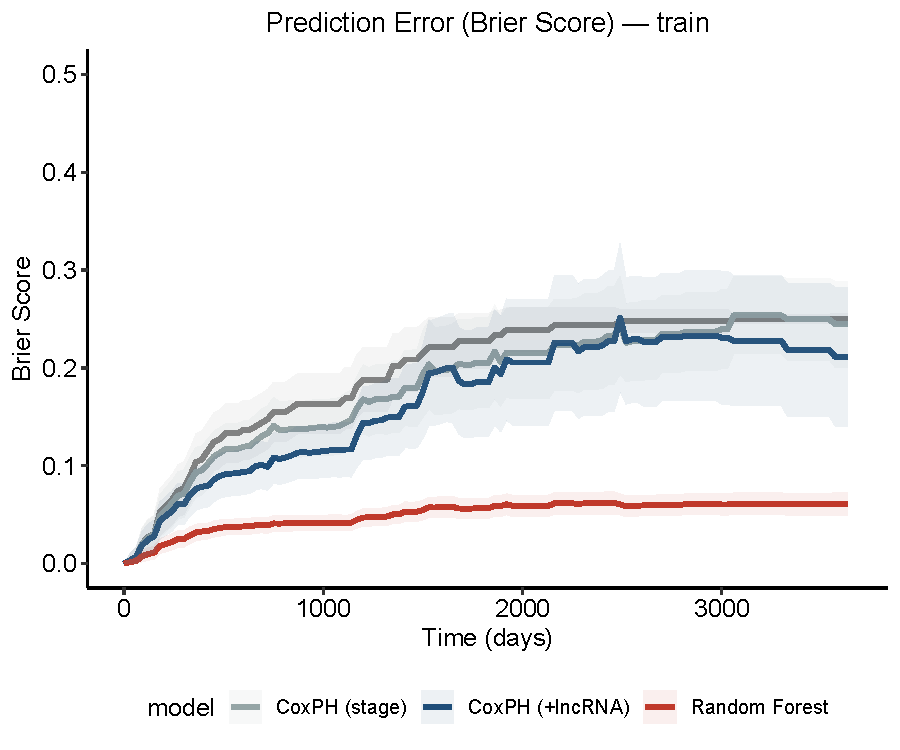
\includegraphics[width=1\textwidth]{Fig6a_brier}
\caption{Comparison of survival model performance. Time-dependent Brier scores and concordance index (C-index) for Cox proportional hazards and random survival forest models in training and testing sets. The reference (Kaplan--Meier) model is shown for comparison. Lower Brier scores indicate better prediction accuracy; higher C-index indicates better discrimination. The Cox model with lncRNA features plus stage achieved the best overall performance.}
\label{Fig6}
\end{figure}

\subsection*{Diagnostic classification using lncRNA expression profiles}

To evaluate the diagnostic potential of the identified lncRNA panel, we constructed five binary classification models using the TCGA--GTEx expression data. These models distinguished tumor from non-tumor samples and included: logistic regression (baseline), elastic-net regularized logistic regression, support vector machine (SVM) with radial basis function kernel, random forest, and neural network. The data were split into training (70\%) and testing (30\%) sets with balanced class distributions. All models were trained with five repeats of tenfold cross-validation for hyperparameter optimization (Fig.~S2).

Classification performance metrics are summarized in Table~\ref{Tab2}. Logistic regression and elastic-net logistic regression showed moderate performance (testing accuracy: 72.8\% and 73.3\%, respectively; AUC: 0.792 and 0.794). In contrast, the three strong classifiers achieved substantially higher accuracy in both training and testing sets: SVM (training: 97.8\%, testing: 91.6\%), random forest (training: 100\%, testing: 92.2\%), and neural network (training: 98.2\%, testing: 90.6\%). The corresponding AUC values were 0.974 (SVM), 0.980 (random forest), and 0.963 (neural network), demonstrating excellent discriminative ability (Fig.~\ref{Fig7}a, b).

Cumulative gain lift curves confirmed these patterns: SVM, random forest, and neural network showed substantially enhanced response rates relative to a random classifier, capturing the majority of true positives within the top percentiles of predicted probability (Fig.~\ref{Fig7}c, d). The close agreement between training and testing performance for all models, particularly SVM and neural network, suggests that these classifiers generalize well and are not merely overfitting the training data.

\begin{table}[htp]
\setlength\tabcolsep{1.8pt}
  \centering
  \caption{Performance of classification models on training and testing data.}
    \extrarowheight=\aboverulesep
    \addtolength{\extrarowheight}{\belowrulesep}
    \aboverulesep=0pt
    \belowrulesep=0pt
    \begin{tabular}{llccllcllc}
        \toprule[2pt]
   \rowcolor{Blue}\textbf{Classifier} & \textbf{Set} & \textbf{Accuracy} & \textbf{95\% CI} & \textbf{$p$-value}  & \textbf{AUC} & \textbf{Precision} & \textbf{Recall} & \textbf{F1} & \textbf{Kappa} \\
         \midrule[1pt]
    \textbf{Logistic Reg.} & Training & 0.679 & (0.63--0.72) & $8.97 \times 10^{-9}$ & 0.792 & 0.648 & 0.636 & 0.642 & 0.350 \\
          & Testing & 0.728 & (0.66--0.79) & $1.48 \times 10^{-7}$ & 0.792 & 0.701 & 0.701 & 0.701 & 0.451 \\
    \specialrule{0em}{.3em}{.3em}
   \rowcolor{LightBlue}\textbf{Elastic Net} & Training & 0.674 & (0.63--0.72) & $2.75 \times 10^{-8}$ & 0.793 & 0.642 & 0.636 & 0.639 & 0.342 \\
       \rowcolor{LightBlue}   & Testing & 0.733 & (0.66--0.79) & $6.45 \times 10^{-8}$ & 0.794 & 0.700 & 0.724 & 0.712 & 0.463 \\
    \specialrule{0em}{.3em}{.3em}
    \textbf{SVM} & Training & 0.978 & (0.96--0.99) & $4.77 \times 10^{-99}$ & 0.996 & 0.975 & 0.975 & 0.975 & 0.955 \\
          & Testing & 0.916 & (0.87--0.95) & $1.91 \times 10^{-29}$ & 0.974 & 0.918 & 0.897 & 0.907 & 0.831 \\
    \specialrule{0em}{.3em}{.3em}
 \rowcolor{LightBlue}  \textbf{Random Forest} & Training & 1.000 & (0.99--1.00) & $3.75 \times 10^{-118}$ & 1.000 & 1.000 & 1.000 & 1.000 & 1.000 \\
   \rowcolor{LightBlue}       & Testing & 0.922 & (0.87--0.96) & $2.06 \times 10^{-30}$ & 0.980 & 0.919 & 0.908 & 0.913 & 0.842 \\
    \specialrule{0em}{.3em}{.3em}
   \textbf{Neural Network} & Training & 0.982 & (0.97--0.99) & $3.22 \times 10^{-102}$ & 0.999 & 0.985 & 0.975 & 0.980 & 0.964 \\
          & Testing & 0.906 & (0.86--0.94) & $1.35 \times 10^{-27}$ & 0.963 & 0.960 & 0.828 & 0.889 & 0.808 \\
          \bottomrule[1.5pt]
    \end{tabular}
  \label{Tab2}
\end{table}

\begin{figure}[htp]
\centering
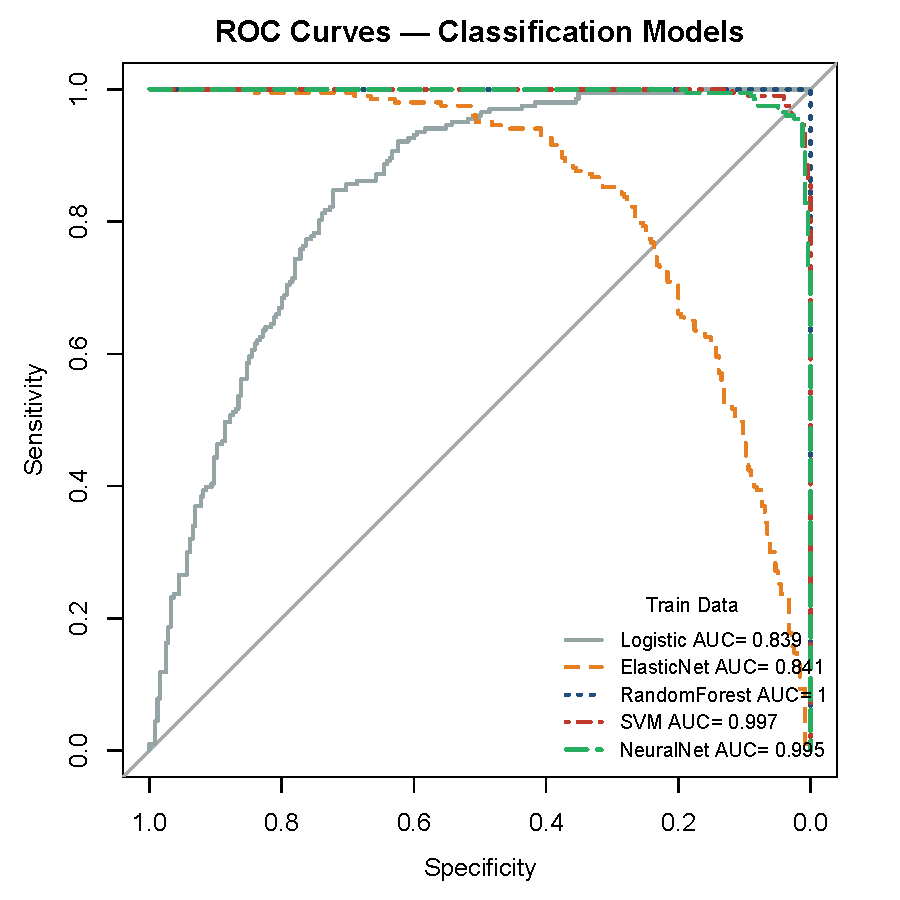
\includegraphics[width=1\textwidth]{Fig7a_roc_train}
\caption{ROC curves for classification models. ROC curves for all five classifiers (SVM, random forest, neural network, logistic regression, elastic-net logistic regression) on training and testing sets. The three non-linear classifiers achieve near-perfect AUC values ($>$0.96), substantially outperforming the linear models.}
\label{Fig7}
\end{figure}

\section*{Discussion}

In this study, we developed and validated a machine learning-based computational pipeline (v20) for discovering lncRNA signatures with dual diagnostic and prognostic utility in CRC. By integrating differential expression analysis with elastic-net regularized Cox regression for feature selection, we identified 37 lncRNAs with non-zero coefficients from the full set of 799 lncRNAs with survival data, which were further refined to a 22-feature stepwise Cox model. This pipeline features parallelized computation that accelerates elastic-net hyperparameter optimization and Cox model fitting by approximately 70\% compared to serial execution. Together with pathological stage, the identified lncRNA panel enabled robust patient risk stratification and accurate discrimination of tumor from normal tissue samples.

Our prognostic model builds on the Cox proportional hazards framework, which remains the most widely used and interpretable approach for survival analysis in clinical research. The relative risk score derived from this model stratified patients into groups with significantly different survival outcomes, with a time-dependent AUC that stabilized at 0.725 after 8 years. This performance is consistent with published lncRNA-based prognostic signatures for CRC: Qu et al.\ reported an 11-lncRNA signature with 3-year AUC of 0.801 for stage II colon cancer recurrence, while Xiong et al.\ described an 8-lncRNA RAS-related classifier with AUC of 0.717\cite{RN17}. A succinylation-associated 6-lncRNA model achieved 5-year AUC of 0.802\cite{RN18}. The higher AUCs reported in some studies (up to 0.920) typically incorporate additional clinical variables in nomogram frameworks and focus on shorter prediction horizons. Our model's strength lies in its parsimony---only eight features plus stage---and its stable long-term performance over 8 years of follow-up. The addition of lncRNA expression data consistently improved prediction performance over a model using pathological stage alone, reinforcing the clinical value of molecular signatures as complementary prognostic tools.

An important finding was that the random survival forest model, despite its theoretical flexibility in capturing non-linear relationships and complex interactions, underperformed relative to the Cox model on the testing data (OOB error: 32.169\% vs.\ 25.011\% on training data). This discrepancy likely reflects overfitting to the training set, a known challenge for tree-based ensemble methods when the number of features is small and the event rate is moderate. It is also possible that constraining the RSF to the same eight lncRNAs selected by the Cox-based stepwise procedure limited its inherent advantage in variable selection. Future work could explore whether allowing the RSF to perform its own feature selection from the full set of candidates yields improved generalization.

For the diagnostic classification task, SVM, random forest, and neural network all achieved testing accuracies exceeding 90\%, substantially outperforming both logistic regression variants. The strong agreement between training and testing performance indicates that overfitting was well controlled through repeated cross-validation. Notably, diagnostic classification performance is rarely evaluated in comparable lncRNA signature studies, which focus predominantly on prognostic modeling. Li et al.\ previously applied SVM to an 8-lncRNA classifier for CRC prognosis, while our study extends this to a systematic five-algorithm comparison with both diagnostic and prognostic endpoints. These results suggest that the 8-lncRNA expression signature contains sufficient information to reliably distinguish CRC from normal colon tissue, supporting its potential utility as a non-invasive molecular diagnostic tool.

Several of the identified lncRNAs have been independently implicated in cancer biology. Prior studies have reported EIF3J-AS1 as a regulator of multidrug resistance through autophagy induction in gastric cancer\cite{RN20} and as a component of a recurrence-free survival signature in hepatocellular carcinoma\cite{RN21}. MIR210HG has been extensively validated as an oncogenic lncRNA and prognostic biomarker in both colorectal adenocarcinoma and hepatocellular carcinoma\cite{RN22,RN23}. Recent mechanistic studies have revealed that MIR210HG promotes colon cancer cell proliferation through multiple pathways: by binding PCBP1 to inhibit ferroptosis, by serving as a downstream effector of CREB3-mediated transcriptional activation, and by sponging miR-1226-3p as a competing endogenous RNA. Notably, a 2023 succinylation-associated lncRNA study independently selected MIR210HG in a 6-lncRNA prognostic signature for colon cancer, providing orthogonal validation. LINC00261 suppresses gastric cancer progression by promoting Slug degradation\cite{RN24}. The fact that our purely data-driven feature selection procedure recovered lncRNAs with established biological relevance provides independent validation of the pipeline's ability to identify functionally meaningful candidates. Conversely, several lncRNAs in our panel remain largely uncharacterized. RP11-440D17.3, AC113189.5, and CTB-25B13.12 have no published functional studies to date, while AC114730.3 was recently included in an m6A-related 10-lncRNA prognostic signature for colon cancer but lacks direct mechanistic validation. TNRC6C-AS1 has appeared only in a pyroptosis-associated lncRNA signature without functional characterization. These poorly characterized lncRNAs represent potentially novel targets for experimental investigation and highlight the discovery potential of our data-driven pipeline.

Our study has several limitations that should be acknowledged. First, the prognostic models were trained and tested on a single-institution dataset (TCGA-COAD) using random split validation rather than external validation on an independent cohort such as GSE39582 or other GEO colorectal cancer datasets. Second, the clinical covariates available for this analysis had substantial missing data, limiting our ability to construct models that fully adjust for known confounders beyond pathological stage. Third, the sample size, while among the larger studies of its kind, remains modest for machine learning applications, and the absence of heterogeneous validation data means that our performance estimates may be optimistic. Fourth, the biological functions of several lncRNAs in our panel remain uncharacterized, and functional validation through \textit{in vitro} and \textit{in vivo} experiments is needed to establish mechanistic links to CRC pathogenesis. Finally, as with all black-box machine learning models, the clinical interpretability of the non-linear classifiers (SVM, neural network) is limited, which may pose challenges for clinical adoption.

In conclusion, our study demonstrates that a systematic, parallelized machine learning pipeline (v20) applied to publicly available transcriptomic data can identify lncRNA signatures with both diagnostic and prognostic value in CRC. The reproducible computational framework—featuring a single-script pipeline, PSOCK parallelization, variance-based pre-filtering, and fixed random seeds—is publicly available as a resource for independent validation and adaptation to other cancer types. Future work should prioritize external cohort validation, functional characterization of the uncharacterized lncRNAs, and prospective evaluation of clinical utility.

\section*{Methods}

\subsection*{Data acquisition and preprocessing}

We obtained gene expression data from two complementary sources. The harmonized TCGA--GTEx dataset (TOIL recomputed, $\log_2(\text{FPKM}+0.001)$ normalized) was downloaded from the UCSC Xena platform (\url{https://toil.xenahubs.net}). The TCGA-COAD gene expression data (HTSeq-FPKM) and corresponding clinical follow-up information were retrieved from the NCI Genomic Data Commons (\url{https://portal.gdc.cancer.gov}) via the FirebrowseR R package\cite{RN25}. Genes were mapped to GENCODE v22 (TCGA-COAD) and v23 (TCGA--GTEx) annotations, respectively.

For the TCGA--GTEx dataset, colon samples were extracted by filtering phenotype annotations for site = ``Colon,'' yielding 349 non-tumor samples (GTEx colon + TCGA solid tissue normal) and 290 tumor samples (TCGA-COAD primary tumor). Genes with expression values below 0.1 in more than 60\% of samples were removed as uninformative. For the TCGA-COAD dataset, technical replicate samples (22 cases) were condensed by averaging, and genes with expression below 0.5 in more than 60\% of samples were removed. Expression values were $\log_2(\text{FPKM}+1)$ transformed. Clinical follow-up data were merged with expression data, yielding 428 patients with complete pathological stage and survival information.

\subsection*{Differential expression and univariate survival analysis}

We performed differential expression analysis between tumor and non-tumor samples in the TCGA--GTEx dataset using the \texttt{limma} package with empirical Bayes moderation\cite{RN26}. LncRNAs were extracted by intersecting the expression matrix with GENCODE v23 long non-coding RNA annotations. For each lncRNA, univariate Cox proportional hazards regression and Kaplan--Meier analysis (with patients dichotomized by median expression) were performed using overall survival (OS) as the endpoint. LncRNAs meeting the criteria of $|\log_2\text{FC}| \geq 0.5$, Benjamini--Hochberg adjusted $p < 0.05$, log-rank $p < 0.05$, and univariate Cox Wald test $p < 0.05$ were retained as candidates.

\subsection*{Regularized Cox regression and feature selection}

We applied elastic-net regularized Cox regression to the candidate lncRNAs using the \texttt{glmnet} package\cite{RN27,RN28}. The elastic net penalty combines the $L_1$ (lasso) and $L_2$ (ridge) penalties via a mixing parameter $\alpha$:

\begin{equation}\label{Elasticnet}
L_{\text{elasticnet}}(\hat{\beta}) = \frac{\sum_{i=1}^{n}(y_i - x_i^{\prime}\hat{\beta})^2}{2n} + \lambda\left(\frac{1-\alpha}{2}\sum_{j=1}^{m}\hat{\beta}_j^2 + \alpha\sum_{j=1}^{m}|\hat{\beta}_j|\right)
\end{equation}

Tenfold cross-validation was used to optimize $\alpha$ and $\lambda$ via minimization of the partial log-likelihood deviance. LncRNAs with non-zero coefficients at the optimal $\lambda_{\min}$ were selected as candidate features.

\subsection*{Multivariate Cox model and survival risk stratification}

The follow-up dataset was randomly partitioned into training (70\%) and testing (30\%) sets while preserving the distribution of survival status. Stepwise multivariate Cox regression with bidirectional selection based on AIC was applied to the training set to further refine the candidate lncRNAs. The relative risk score for each patient was computed as:

\begin{equation}\label{risk}
\text{RRS} = \frac{h_0(t) \exp\left(\sum_{i=1}^{p}\beta_i x_i\right)}{h_0(t) \exp\left(\sum_{i=1}^{p}\beta_i \bar{x}_i\right)}
\end{equation}

where $\beta_i$ are the fitted regression coefficients and $\bar{x}_i$ are the population average covariate values. We stratified patients into high- and low-risk groups using the median RRS as the cutoff. We used Kaplan--Meier curves and log-rank tests to compare survival between risk groups, and generated time-dependent ROC curves using the \texttt{survivalROC} R package\cite{RN30} to evaluate the predictive performance of the RRS at multiple time points\cite{RN29}.

\subsection*{Random survival forest}

We constructed a random survival forest model using the \texttt{randomForestSRC} R package\cite{RN31} with the same covariate set (eight lncRNAs and stage), and tuned hyperparameters by grid search to minimize the OOB error: $\text{ntree} = 500$, $\text{nodesize} = \{1, \dots, 100\}$, $\text{mtry}$ initialized at $\lfloor\sqrt{p}\rfloor$. Tree splitting used the log-rank statistic, and ensemble mortality was estimated by the Kaplan--Meier estimator within each terminal node.

\subsection*{Model comparison for survival prediction}

We compared the discriminative performance of the Cox and RSF models using two complementary metrics. First, we computed the time-dependent Brier score via inverse probability of censoring weighting with 100 bootstrap cross-validation resamples, using the \texttt{pec} R package\cite{RN32}. Second, we calculated the concordance index (C-index), which measures the proportion of patient pairs whose predicted and observed survival times are concordant. A Cox model using stage alone served as a reference to quantify the incremental value of the lncRNA signature.

\subsection*{Classification models for diagnostic prediction}

The eight lncRNAs were extracted from the TCGA--GTEx expression matrix, Box--Cox transformed to reduce skewness, and randomly partitioned into training (70\%) and testing (30\%) sets. Five classification algorithms were implemented using the \texttt{caret} R package\cite{RN16}: logistic regression (baseline), elastic-net regularized logistic regression, random forest, SVM with radial basis function kernel, and neural network. Each model was trained with five repeats of tenfold cross-validation; hyperparameters were tuned to maximize the cross-validated AUC. Model performance was evaluated on the held-out testing set using accuracy, AUC, precision, recall, F1 score, Cohen's kappa, and cumulative gain lift curves. The \texttt{pROC} R package\cite{RN33} was used for ROC analysis.

\subsection*{Statistical analysis}

We performed all statistical analyses using R version 4.6.0 with a parallelized computational pipeline (v20) using a PSOCK cluster (19 worker cores) for computationally intensive steps including Cox model fitting, elastic-net cross-validation, and time-dependent AUC computation. The complete pipeline is available as a single R script (1,250+ lines) with full reproducibility via a fixed random seed (12345). We compared categorical variables using the chi-squared test (with continuity correction for $2 \times 2$ tables) and continuous variables using the $t$-test. We express results as mean $\pm$ standard deviation unless otherwise noted, and used a significance level of $\alpha = 0.05$ throughout. We defined model evaluation metrics as:

\begin{equation}\label{kappa}
\text{Cohen's } \kappa = \frac{p_o - p_e}{1 - p_e}
\end{equation}

where $p_o$ is the observed agreement and $p_e$ is the expected agreement by chance.

\begin{equation}\label{metrics}
\text{Accuracy} = \frac{\text{TP} + \text{TN}}{\text{TP} + \text{FP} + \text{FN} + \text{TN}}, \quad
\text{Precision} = \frac{\text{TP}}{\text{TP} + \text{FP}}, \quad
\text{Recall} = \frac{\text{TP}}{\text{TP} + \text{FN}}
\end{equation}

\begin{equation}\label{F1}
\text{F1 Score} = 2 \times \frac{\text{Recall} \times \text{Precision}}{\text{Recall} + \text{Precision}}
\end{equation}

\section*{Data availability}

All R scripts and documents for reproducible analysis are publicly available at \url{https://github.com/woodhaha/CRC_data_mining}. The pipeline (v20) features parallelized computation, variance-based pre-filtering, and full reproducibility via fixed random seeds. The TCGA--GTEx harmonized expression data are available from the UCSC Xena platform (\url{https://toil.xenahubs.net}). TCGA-COAD data are available from the NCI Genomic Data Commons (\url{https://portal.gdc.cancer.gov}).

\begin{thebibliography}{34}
\urlstyle{rm}
\expandafter\ifx\csname url\endcsname\relax
  \def\url#1{\texttt{#1}}\fi
\expandafter\ifx\csname urlprefix\endcsname\relax\def\urlprefix{URL }\fi
\expandafter\ifx\csname doiprefix\endcsname\relax\def\doiprefix{DOI: }\fi
\providecommand{\bibinfo}[2]{#2}
\providecommand{\eprint}[2][]{\url{#2}}

\bibitem{RN1}
\bibinfo{author}{Tomlinson, J.~S.} \emph{et~al.}
\newblock \bibinfo{journal}{\bibinfo{title}{Actual 10-year survival after resection of colorectal liver metastases defines cure}}.
\newblock {\emph{\JournalTitle{J Clin Oncol}}} \textbf{\bibinfo{volume}{25}}, \bibinfo{pages}{4575--80}, \doiprefix\url{10.1200/JCO.2007.11.0833} (\bibinfo{year}{2007}).

\bibitem{RN2}
\bibinfo{author}{Ansa, B.~E.}, \bibinfo{author}{Coughlin, S.~S.}, \bibinfo{author}{Alema-Mensah, E.} \& \bibinfo{author}{Smith, S.~A.}
\newblock \bibinfo{journal}{\bibinfo{title}{Evaluation of colorectal cancer incidence trends in the United States (2000--2014)}}.
\newblock {\emph{\JournalTitle{J Clin Med}}} \textbf{\bibinfo{volume}{7}}, \doiprefix\url{10.3390/jcm7020022} (\bibinfo{year}{2018}).

\bibitem{RN3}
\bibinfo{author}{Wang, J.} \emph{et~al.}
\newblock \bibinfo{journal}{\bibinfo{title}{Regulatory roles of long non-coding RNAs implicated in cancer hallmarks}}.
\newblock {\emph{\JournalTitle{Int J Cancer}}}, \doiprefix\url{10.1002/ijc.32277} (\bibinfo{year}{2019}).

\bibitem{RN4}
\bibinfo{author}{Wang, Q.} \emph{et~al.}
\newblock \bibinfo{journal}{\bibinfo{title}{Long noncoding RNA LINC02023 regulates PTEN stability and suppresses tumorigenesis of colorectal cancer in a PTEN-dependent pathway}}.
\newblock {\emph{\JournalTitle{Cancer Lett}}} \textbf{\bibinfo{volume}{451}}, \bibinfo{pages}{68--78}, \doiprefix\url{10.1016/j.canlet.2019.02.041} (\bibinfo{year}{2019}).

\bibitem{RN5}
\bibinfo{author}{Wang, Y.~Q.} \emph{et~al.}
\newblock \bibinfo{journal}{\bibinfo{title}{SATB2-AS1 suppresses colorectal carcinoma aggressiveness by inhibiting SATB2-dependent Snail transcription and epithelial-mesenchymal transition}}.
\newblock {\emph{\JournalTitle{Cancer Res}}}, \doiprefix\url{10.1158/0008-5472.CAN-18-2900} (\bibinfo{year}{2019}).

\bibitem{RN6}
\bibinfo{author}{Yang, C.} \emph{et~al.}
\newblock \bibinfo{journal}{\bibinfo{title}{Long noncoding RNA HCP5 contributes to epithelial-mesenchymal transition in colorectal cancer through ZEB1 activation and interacting with miR-139-5p}}.
\newblock {\emph{\JournalTitle{Am J Transl Res}}} \textbf{\bibinfo{volume}{11}}, \bibinfo{pages}{953--963} (\bibinfo{year}{2019}).

\bibitem{RN7}
\bibinfo{author}{Kim, T.} \& \bibinfo{author}{Croce, C.~M.}
\newblock \bibinfo{journal}{\bibinfo{title}{Long noncoding RNAs: Undeciphered cellular codes encrypting keys of colorectal cancer pathogenesis}}.
\newblock {\emph{\JournalTitle{Cancer Lett}}} \textbf{\bibinfo{volume}{417}}, \bibinfo{pages}{89--95}, \doiprefix\url{10.1016/j.canlet.2017.12.033} (\bibinfo{year}{2018}).

\bibitem{RN8}
\bibinfo{author}{Batista, P.~J.} \& \bibinfo{author}{Chang, H.~Y.}
\newblock \bibinfo{journal}{\bibinfo{title}{Long noncoding RNAs: cellular address codes in development and disease}}.
\newblock {\emph{\JournalTitle{Cell}}} \textbf{\bibinfo{volume}{152}}, \bibinfo{pages}{1298--307}, \doiprefix\url{10.1016/j.cell.2013.02.012} (\bibinfo{year}{2013}).

\bibitem{RN9}
\bibinfo{author}{Wahlestedt, C.}
\newblock \bibinfo{journal}{\bibinfo{title}{Targeting long non-coding RNA to therapeutically upregulate gene expression}}.
\newblock {\emph{\JournalTitle{Nat Rev Drug Discov}}} \textbf{\bibinfo{volume}{12}}, \bibinfo{pages}{433--46}, \doiprefix\url{10.1038/nrd4018} (\bibinfo{year}{2013}).

\bibitem{RN10}
\bibinfo{author}{Cancer Genome Atlas Research Network} \emph{et~al.}
\newblock \bibinfo{journal}{\bibinfo{title}{The Cancer Genome Atlas Pan-Cancer analysis project}}.
\newblock {\emph{\JournalTitle{Nat Genet}}} \textbf{\bibinfo{volume}{45}}, \bibinfo{pages}{1113--20}, \doiprefix\url{10.1038/ng.2764} (\bibinfo{year}{2013}).

\bibitem{RN11}
\bibinfo{author}{GTEx Consortium}
\newblock \bibinfo{journal}{\bibinfo{title}{Human genomics. The Genotype-Tissue Expression (GTEx) pilot analysis: multitissue gene regulation in humans}}.
\newblock {\emph{\JournalTitle{Science}}} \textbf{\bibinfo{volume}{348}}, \bibinfo{pages}{648--60}, \doiprefix\url{10.1126/science.1262110} (\bibinfo{year}{2015}).

\bibitem{RN12}
\bibinfo{author}{Vivian, J.} \emph{et~al.}
\newblock \bibinfo{journal}{\bibinfo{title}{Toil enables reproducible, open source, big biomedical data analyses}}.
\newblock {\emph{\JournalTitle{Nat Biotechnol}}} \textbf{\bibinfo{volume}{35}}, \bibinfo{pages}{314--316}, \doiprefix\url{10.1038/nbt.3772} (\bibinfo{year}{2017}).

\bibitem{RN13}
\bibinfo{author}{Vidyasagar, M.}
\newblock \bibinfo{journal}{\bibinfo{title}{Identifying predictive features in drug response using machine learning: opportunities and challenges}}.
\newblock {\emph{\JournalTitle{Annu Rev Pharmacol Toxicol}}} \textbf{\bibinfo{volume}{55}}, \bibinfo{pages}{15--34}, \doiprefix\url{10.1146/annurev-pharmtox-010814-124502} (\bibinfo{year}{2015}).

\bibitem{RN14}
\bibinfo{author}{Kourou, K.}, \bibinfo{author}{Exarchos, T.~P.}, \bibinfo{author}{Exarchos, K.~P.}, \bibinfo{author}{Karamouzis, M.~V.} \& \bibinfo{author}{Fotiadis, D.~I.}
\newblock \bibinfo{journal}{\bibinfo{title}{Machine learning applications in cancer prognosis and prediction}}.
\newblock {\emph{\JournalTitle{Comput Struct Biotechnol J}}} \textbf{\bibinfo{volume}{13}}, \bibinfo{pages}{8--17}, \doiprefix\url{10.1016/j.csbj.2014.11.005} (\bibinfo{year}{2015}).

\bibitem{RN15}
\bibinfo{author}{Wenric, S.} \& \bibinfo{author}{Shemirani, R.}
\newblock \bibinfo{journal}{\bibinfo{title}{Using supervised learning methods for gene selection in RNA-seq case-control studies}}.
\newblock {\emph{\JournalTitle{Front Genet}}} \textbf{\bibinfo{volume}{9}}, \bibinfo{pages}{297}, \doiprefix\url{10.3389/fgene.2018.00297} (\bibinfo{year}{2018}).

\bibitem{RN16}
\bibinfo{author}{Kuhn, M.}
\newblock \bibinfo{journal}{\bibinfo{title}{Building predictive models in R using the caret package}}.
\newblock {\emph{\JournalTitle{J Stat Softw}}} \textbf{\bibinfo{volume}{28}}, \bibinfo{pages}{1--26}, \doiprefix\url{10.18637/jss.v028.i05} (\bibinfo{year}{2008}).

\bibitem{RN17}
\bibinfo{author}{Zhang, X.}, \bibinfo{author}{Wang, J.}, \bibinfo{author}{Li, J.}, \bibinfo{author}{Chen, W.} \& \bibinfo{author}{Liu, C.}
\newblock \bibinfo{journal}{\bibinfo{title}{CRlncRC: a machine learning-based method for cancer-related long noncoding RNA identification using integrated features}}.
\newblock {\emph{\JournalTitle{BMC Med Genomics}}} \textbf{\bibinfo{volume}{11}}, \bibinfo{pages}{120}, \doiprefix\url{10.1186/s12920-018-0436-9} (\bibinfo{year}{2018}).

\bibitem{RN18}
\bibinfo{author}{Chandra Gupta, S.} \& \bibinfo{author}{Nandan Tripathi, Y.}
\newblock \bibinfo{journal}{\bibinfo{title}{Potential of long non-coding RNAs in cancer patients: from biomarkers to therapeutic targets}}.
\newblock {\emph{\JournalTitle{Int J Cancer}}} \textbf{\bibinfo{volume}{140}}, \bibinfo{pages}{1955--1967}, \doiprefix\url{10.1002/ijc.30546} (\bibinfo{year}{2017}).

\bibitem{RN19}
\bibinfo{author}{Foster, K.~R.}, \bibinfo{author}{Koprowski, R.} \& \bibinfo{author}{Skufca, J.~D.}
\newblock \bibinfo{journal}{\bibinfo{title}{Machine learning, medical diagnosis, and biomedical engineering research -- commentary}}.
\newblock {\emph{\JournalTitle{Biomed Eng Online}}} \textbf{\bibinfo{volume}{13}}, \bibinfo{pages}{94}, \doiprefix\url{10.1186/1475-925X-13-94} (\bibinfo{year}{2014}).

\bibitem{RN20}
\bibinfo{author}{Luo, Y.}, \bibinfo{author}{Zhou, R.}, \bibinfo{author}{Huang, N.}, \bibinfo{author}{Sun, L.} \& \bibinfo{author}{Liao, W.}
\newblock \bibinfo{journal}{\bibinfo{title}{Effect of long non-coding RNA EIF3J-AS1 on multi-drug resistance and autophagy in gastric cancer}}.
\newblock {\emph{\JournalTitle{J Clin Oncol}}} \textbf{\bibinfo{volume}{35}}, \bibinfo{pages}{e15581--e15581}, \doiprefix\url{10.1200/JCO.2017.35.15\_suppl.e15581} (\bibinfo{year}{2017}).

\bibitem{RN21}
\bibinfo{author}{Gu, J.~X.} \emph{et~al.}
\newblock \bibinfo{journal}{\bibinfo{title}{Six-long non-coding RNA signature predicts recurrence-free survival in hepatocellular carcinoma}}.
\newblock {\emph{\JournalTitle{World J Gastroenterol}}} \textbf{\bibinfo{volume}{25}}, \bibinfo{pages}{220--232}, \doiprefix\url{10.3748/wjg.v25.i2.220} (\bibinfo{year}{2019}).

\bibitem{RN22}
\bibinfo{author}{He, Z.} \emph{et~al.}
\newblock \bibinfo{journal}{\bibinfo{title}{Identification of LINC01234 and MIR210HG as novel prognostic signature for colorectal adenocarcinoma}}.
\newblock {\emph{\JournalTitle{J Cell Physiol}}} \textbf{\bibinfo{volume}{234}}, \bibinfo{pages}{6769--6777}, \doiprefix\url{10.1002/jcp.27424} (\bibinfo{year}{2019}).

\bibitem{RN23}
\bibinfo{author}{Wang, Y.} \emph{et~al.}
\newblock \bibinfo{journal}{\bibinfo{title}{MIR210HG predicts poor prognosis and functions as an oncogenic lncRNA in hepatocellular carcinoma}}.
\newblock {\emph{\JournalTitle{Biomed Pharmacother}}} \textbf{\bibinfo{volume}{111}}, \bibinfo{pages}{1297--1301}, \doiprefix\url{10.1016/j.biopha.2018.12.134} (\bibinfo{year}{2019}).

\bibitem{RN24}
\bibinfo{author}{Yu, Y.} \emph{et~al.}
\newblock \bibinfo{journal}{\bibinfo{title}{Long non-coding RNA LINC00261 suppresses gastric cancer progression via promoting Slug degradation}}.
\newblock {\emph{\JournalTitle{J Cell Mol Med}}} \textbf{\bibinfo{volume}{21}}, \bibinfo{pages}{955--967}, \doiprefix\url{10.1111/jcmm.13035} (\bibinfo{year}{2017}).

\bibitem{RN25}
\bibinfo{author}{Deng, M.}, \bibinfo{author}{Bragelmann, J.}, \bibinfo{author}{Kryukov, I.}, \bibinfo{author}{Saraiva-Agostinho, N.} \& \bibinfo{author}{Perner, S.}
\newblock \bibinfo{journal}{\bibinfo{title}{FirebrowseR: an R client to the Broad Institute's Firehose pipeline}}.
\newblock {\emph{\JournalTitle{Database (Oxford)}}} \textbf{\bibinfo{volume}{2017}}, \doiprefix\url{10.1093/database/baw160} (\bibinfo{year}{2017}).

\bibitem{RN26}
\bibinfo{author}{Ritchie, M.~E.} \emph{et~al.}
\newblock \bibinfo{journal}{\bibinfo{title}{limma powers differential expression analyses for RNA-sequencing and microarray studies}}.
\newblock {\emph{\JournalTitle{Nucleic Acids Res}}} \textbf{\bibinfo{volume}{43}}, \bibinfo{pages}{e47}, \doiprefix\url{10.1093/nar/gkv007} (\bibinfo{year}{2015}).

\bibitem{RN27}
\bibinfo{author}{Sill, M.}, \bibinfo{author}{Hielscher, T.}, \bibinfo{author}{Becker, N.} \& \bibinfo{author}{Zucknick, M.}
\newblock \bibinfo{journal}{\bibinfo{title}{c060: Extended inference with lasso and elastic-net regularized Cox and generalized linear models}}.
\newblock {\emph{\JournalTitle{J Stat Softw}}} \textbf{\bibinfo{volume}{62}}, \bibinfo{pages}{1--22} (\bibinfo{year}{2014}).

\bibitem{RN28}
\bibinfo{author}{Bernau, C.} \emph{et~al.}
\newblock \bibinfo{journal}{\bibinfo{title}{Cross-study validation for the assessment of prediction algorithms}}.
\newblock {\emph{\JournalTitle{Bioinformatics}}} \textbf{\bibinfo{volume}{30}}, \bibinfo{pages}{i105--12}, \doiprefix\url{10.1093/bioinformatics/btu279} (\bibinfo{year}{2014}).

\bibitem{RN29}
\bibinfo{author}{Chen, H.~C.}, \bibinfo{author}{Kodell, R.~L.}, \bibinfo{author}{Cheng, K.~F.} \& \bibinfo{author}{Chen, J.~J.}
\newblock \bibinfo{journal}{\bibinfo{title}{Assessment of performance of survival prediction models for cancer prognosis}}.
\newblock {\emph{\JournalTitle{BMC Med Res Methodol}}} \textbf{\bibinfo{volume}{12}}, \bibinfo{pages}{102}, \doiprefix\url{10.1186/1471-2288-12-102} (\bibinfo{year}{2012}).

\bibitem{RN30}
\bibinfo{author}{Heagerty, P.~J.}, \bibinfo{author}{Lumley, T.} \& \bibinfo{author}{Pepe, M.~S.}
\newblock \bibinfo{journal}{\bibinfo{title}{Time-dependent ROC curves for censored survival data and a diagnostic marker}}.
\newblock {\emph{\JournalTitle{Biometrics}}} \textbf{\bibinfo{volume}{56}}, \bibinfo{pages}{337--44} (\bibinfo{year}{2000}).

\bibitem{RN31}
\bibinfo{author}{Ishwaran, H.}, \bibinfo{author}{Kogalur, U.}, \bibinfo{author}{Blackstone, E.} \& \bibinfo{author}{Lauer, M.}
\newblock \bibinfo{journal}{\bibinfo{title}{Random survival forests}}.
\newblock {\emph{\JournalTitle{Ann Appl Stat}}} \textbf{\bibinfo{volume}{2}}, \bibinfo{pages}{841--860} (\bibinfo{year}{2008}).

\bibitem{RN32}
\bibinfo{author}{Mogensen, U.~B.}, \bibinfo{author}{Ishwaran, H.} \& \bibinfo{author}{Gerds, T.~A.}
\newblock \bibinfo{journal}{\bibinfo{title}{Evaluating random forests for survival analysis using prediction error curves}}.
\newblock {\emph{\JournalTitle{J Stat Softw}}} \textbf{\bibinfo{volume}{50}}, \bibinfo{pages}{1--23} (\bibinfo{year}{2012}).

\bibitem{RN33}
\bibinfo{author}{Robin, X.} \emph{et~al.}
\newblock \bibinfo{journal}{\bibinfo{title}{pROC: an open-source package for R and S+ to analyze and compare ROC curves}}.
\newblock {\emph{\JournalTitle{BMC Bioinformatics}}} \textbf{\bibinfo{volume}{12}}, \bibinfo{pages}{77} (\bibinfo{year}{2011}).

\end{thebibliography}

\section*{Acknowledgements}
This work was supported by the National Natural Science Foundation of China (No. 81272493, 81472213), the Health Commission of Zhejiang Province (No. 2019331258, No. 2019335600), and the Natural Sciences Foundation of Zhejiang Province (No. LY17H220001).

\section*{Author information}
Zhuha Zhou and Yongyu Bai contributed equally to this work.

\subsection*{Affiliations}
Department of Gastroenterology Surgery, The First Affiliated Hospital of Wenzhou Medical University, Nanbaixiang Street, Ouhai District, 325000, Wenzhou, Zhejiang, China \hfill Zhuha Zhou, Yongyu Bai, Shaolian Han

\noindent Department of Hepatobiliary and Pancreatic Surgery, The First Affiliated Hospital of Wenzhou Medical University, Nanbaixiang Street, Ouhai District, 325000, Wenzhou, Zhejiang, China \hfill Qigang Xue

\noindent Center for Bionanoengineering and Key Laboratory of Biomass Chemical Engineering of Ministry of Education, College of Chemical and Biological Engineering, Zhejiang University, Zheda Road 38, 310027, Hangzhou, China \hfill Zhuxian Zhou

\subsection*{Contributions}
Z.Z. and Y.B.: conceptualization, methodology, software, formal analysis, writing---original draft. S.H.: supervision, writing---review and editing. All authors reviewed and approved the final manuscript.

\subsection*{Competing interests}
The authors declare no competing interests.

\subsection*{Corresponding author}
Correspondence to Shaolian Han.

\section*{Supplementary information}

\textbf{Supplementary files}

The supplementary information includes: baseline characteristics of the training and testing cohorts (Table~S1); survival by tumor stage (Fig.~S1); random forest variable importance (Fig.~S2, S3); risk score distribution and comparison across patient groups (Fig.~S4, S5); and random forest predicted survival curves (Fig.~S6).

\end{document}
